% ========== Chapter 3
\chapter{\texttt{dms-view}: Interactive visualization tool for deep mutational scanning experiments}

Sarah Hilton*, John Huddleston*, Allison Black, Khrystyna North, Adam Dingens, Trevor Bedford, and Jesse Bloom.

(* equal contribution)

\clearpage

\section{Summary and Purpose}

One challenge in studying proteins is that the effect of amino-acid changes are idiosyncratic across the length of the gene.
However, recent technological developments in the form of a high-throughput functional assay called Deep Mutational Scanning (DMS)~\cite{fowler2014deep}, make it possible to experimentally measure the effect of all amino-acid mutations to a protein.
Over the past five years, this flexible assay has been used to study dozens of different proteins~\cite{esposito2019mavedb} and answer a variety of research questions.
For example, DMS approaches have been used for protein engineering~\cite{wrenbeck2017deep}, understanding the human immune response to viruses~\cite{lee2019mapping}, and to potentially interpret human variation in a clinical setting\cite{starita2017variant, gelman2019recommendations}.
Accompanying this explosion in DMS studies has been the development of software tools~\cite{bloom2015software,rubin2017statistical} and databases~\cite{esposito2019mavedb} to standardize DMS analysis and facilitate data sharing.
However, the power of a DMS study is only fully leveraged when the experimental results are summarized, integrated, and visualized with other data, such the 3d protein structure and natural sequence data.

Here we describe \texttt{dms-view} (\url{https://dms-view.github.io/}), a flexible, web-based, interactive visualization tool for deep mutational scanning experiments written in JavaScript and D3 (\url{https://d3js.org}).
\texttt{dms-view} links site-level and mutation-level results from a DMS to a 3D protein structure.
The user can interactively select sites of interest to reveal the mutation-level details and view the sites on the protein structure.
\texttt{dms-view} tracks both the input data information and the user selections in the URL.
This allows the user to save their selections or send a specific view to collaborator.
Importantly, \texttt{dms-view} is designed with a flexible input data file so the user can display custom site- and mutation-level metrics and incorporate non-DMS data, such amino-acid frequencies in nature.

\section{How to use \texttt{dms-view}}

\texttt{dms-view} is a web-based visualization tool hosted by GitHub Pages(\url{https://pages.github.com/}).
In this section, we will briefly explain how \texttt{dms-view} is laid out, the interaction tools available to the user and how to format and upload a new dataset.
For more information on any of these topics, please see the documentation at \url{https://dms-view.github.io/docs}.

\subsection{\texttt{dms-view} layout}

Users can access \texttt{dms-view} at \url{https://dms-view.github.io}.
The tool is broken into a data section at the top and a metadata section at the bottom (Fig~\ref{fig:layout}A).

The data section displays the user specified data (see data upload section below) in three panels: the site dot plot panel, the mutation logoplot panel, and the protein structure panelFig~\ref{fig:layout}B.
When sites are selected in the site dot plot panel, the individual mutation values are shown in the mutation logoplot panel below and highlighted on the protein structure to the right.

The metadata section is at the bottom of the page.
The user can use this section to explain the experimental setup, acknowledge data sources, hold notes about a particular analysis or another relevant information.

\subsection{interaction tool}

The user can interact with \texttt{dms-view} visualizations through selections, navigation options, and toggling between different datasets.

\subsubsection{selections}

The main way the user interacts with \texttt{dms-view} is by selecting or deselecting points of interest.
Below we list the four ways to modify the site selections.

\begin{itemize}
  \item Clicking on a site: The user can click on a site to select it and click again to deselect.
  \item Brushing a site(s): The user can brush several sites at once by clicking, holding, and swiping the mouse. The sites within the brush box will be select. To change the brush to a ``deselect" brush, the user can toggle the radio buttons or use the keyboard shortcut and hold down shift while they brush.
  \item Listing a site(s): The user can select or deselect sites by adding or removing them from the selected site form field respectively. The selected site field is a comma-separated list without leading or trailing spaces. This list is automatically updated with sites selected by clicking and/or brushing.
  \item Clicking the ``clear selections" button: The user can clear all selected sites by clicking on the ``clear selections" button.
\end{itemize}

\subsubsection{navigation}
\texttt{dms-view} has two features to help the user find a specific site in the dot plot.
Hovering over a dot in the site dot plot will reveal a tooltip with information about the site such as its identity, its value, and the wildtype amino-acid at that site.
The user can also zoom in to a specific area of the site dot plot using the zoom bar.

\subsubsection{changing datasets}

The user can toggle between different datasets using a combination of the site-level, mutation level, and condition dropdown menu.
All three of these menus are auto populated with values from the user-created data file.

\subsection{data upload}

The user specifies the three files required by \texttt{dms-view} (the data file, the protein structure file, and the metadata file) using the form fields on the main page.
In order to upload a new dataset, the user simple changes the URL in the form field.
\texttt{dms-view} tracks the data file, protein structure and metadata file URLs in its own URL which allows the user to share a complete view of the tool by simple sending the URL.

Below, we briefly explain the form and contents of the three required input files.
For more information and complete examples, please see the documentation at \url{https://dms-view.github.io/docs/dataupload}.
Finally, while \texttt{dms-view} was designed for DMS experiments, the tool will display any data that follows the data file, protein structure file, and metadata file formats.

\subsubsection{data file}

The data file is the main source of data for \texttt{dms-view}.
This csv (comma separated values) file contains the measurements for the site dot plot, the measurements for the mutation logoplot, and the map between the site plot numbering and the protein structure numbering.
The condition, site-metric, and mutation-metric dropdown menus will be autopopulated using the values in this file.
For complete explanation of the data file, including the required columns and examples, please see the documentation at \url{https://dms-view.github.io/docs/dataupload}.

\subsubsection{protein structure file}

The protein structure file must be a standard protein databank (pdb) file.
For complete explanation of the protein structure file, including examples, please see the documentation at \url{https://dms-view.github.io/docs/dataupload}.

\subsubsection{metadata file}

The metadata file is a markdown file.
The user can use this file to explain an experiment, acknowledge contributors, or other notes.
For complete explanation of the metadata file, including examples, please see the documentation at \url{https://dms-view.github.io/docs/dataupload}.

\section{Examples}

Below are examples of two different published datasets analyzed using \texttt{dms-view}.

\subsection{Mapping Influenza Virus escape from human sera}

Using a deep mutational scanning approach, Lee \textit{et al.}, 2019~\cite{lee2019mapping} measured the ability of every single amino-acid mutation in the Influenza Virus surface protein hemagglutinin to escape the sera of both humans and infected ferrets.
For more information on the experimental setup, see the paper~\cite{lee2019mapping} or the GitHub repo(\url{https://github.com/jbloomlab/map_flu_serum_Perth2009_H3_HA}).

In this example, the conditions are the different human or ferret sera used for the selections.
The site- and mutation-level metrics are different summaries of \textit{differential selection}(\url{https://jbloomlab.github.io/dms_tools2/diffsel.html}), where higher values indicate more escape from the sera.

Lee and colleagues asked two questions in their paper which can be easily explored using \texttt{dms-view}.

\begin{enumerate}
  \item Are the same sites selected by the human and the ferret sera? (compare site-level and mutation-level metric values for specific sites between different conditions)
  \item Where on the protein structure are the highly selected sites located? (view sites on the protein structure)
\end{enumerate}

\subsubsection{Comparing site-level and mutation-level metric values for specific sites between conditions}

To address this question using \texttt{dms-view}, we selected the mostly highly targted sites (144, 159, 193, and 222) for the human sera condition ``Age 21 2010" (Fig~\ref{fig:human-vs-ferrets}A).
We can then use the condition dropdown menu to toggle between the other human and ferret sera.
Since the highlighted sites remain after the condition is changed, we can easily see if the same sites are highly targeted in different samples.

In Fig~\ref{fig:human-vs-ferrets}B, we can see that 2 of the sites selected by the human sera ``Age 21 2010" are also targeted by the ferret sera 2.
To explore this question in more detail, please see the \texttt{dms-view} link XX.

\subsubsection{Where on the protein structure are the highly selected sites located?}

To address this question using \texttt{dms-view}, we selected the most highly targeted sites (144, 159, 193, and 222) for the human sera condition ``Age 21 2010" to highlight them on the protein structure.

In Fig~\ref{fig:human-vs-ferrets}A, we can see that these sites cluster on the ``head" of the hemagglutinin (cite x), which is known to be a common target of the human immune system.

\subsection{maybe **gasp** a non-Bloom lab dataset?}

I was thinking of maybe one of the datasets from Doug Fowler's group, such as Kenney's PTEN dataset.

\section{Code Availability}

All of the code, docs, and example data are hosted on GitHub.

\begin{itemize}
  \item To view the tool, visit \url{https://dms-view.github.io}
  \item To view the tool's source code, visit \url{https://github.com/dms-view/dms-view.github.io}
  \item To view the documentation, visit \url{https://dms-view.github.io/docs}
  \item to view example datasets, visit \url{https://dms-view.github.io/docs/casestudies/}
\end{itemize}

\section{Acknowledgements}

This work started as the final project for UW class CSE 512 Data Visualization as a part of the UW eScience Advanced Data Science Option curriculum and we would like to thank Dr. Jeffrey Heer, Halden Lin, and Jane Hoffswell for their input on the initial design.
Thank you to Bloom and Bedford lab members for their generosity providing feedback, data, and time for testing.

% ========== Figures

\newpage
\begin{figure}[h!]
\centerline{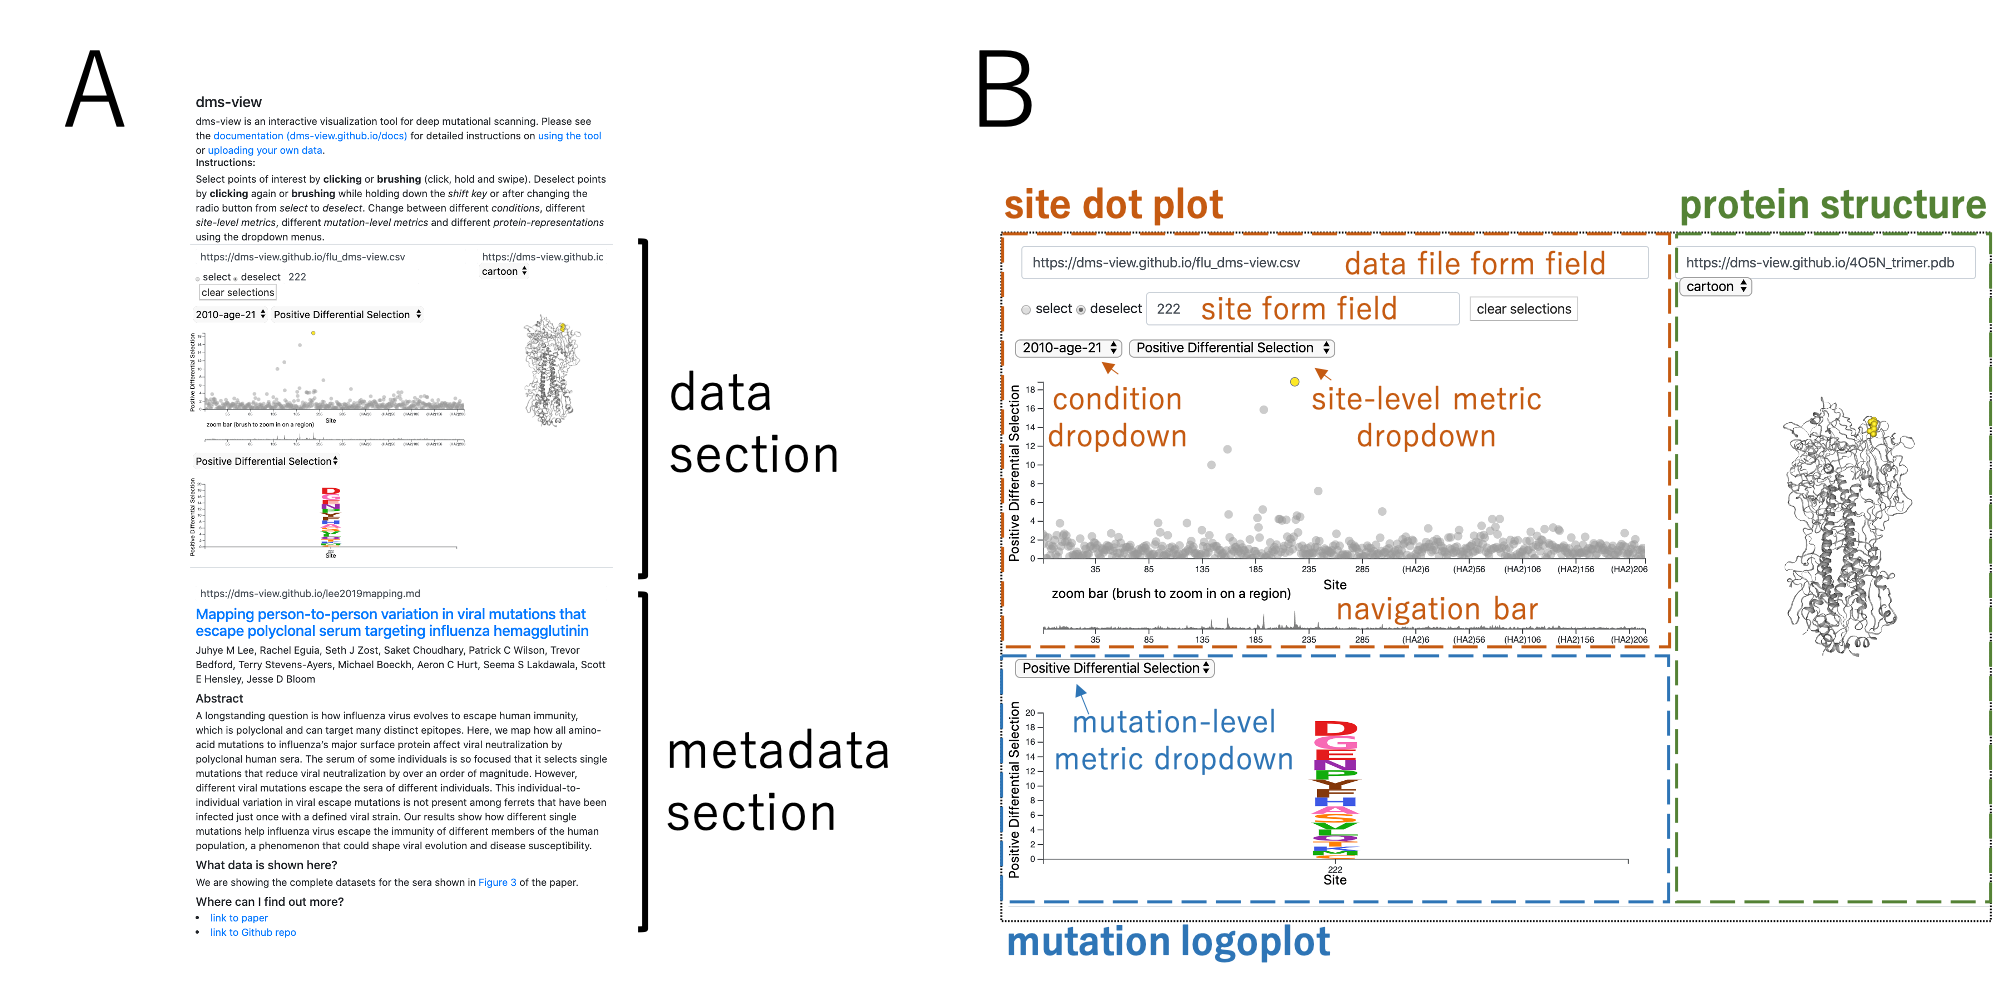
\includegraphics[width=0.90\textwidth]{../fig/layout.png}}
\caption[\texttt{dms-view} layout]{
\label{fig:layout}
\textbf{Main sections and features of the \texttt{dms-view} tool.}
{\bf (A)} \texttt{dms-view} is broken into a data section with the interactive plots at the top and a metadata section for notes and description at the bottom.
{\bf (B)} The \texttt{dms-view} data section has three panels: the site dot plot panel, the mutation logoplot panel, and the protein structure panel.
The interactive features for selecting sites and navigating are in the site dot plot panel.
}
\end{figure}

\newpage
\begin{figure}[h!]
\centerline{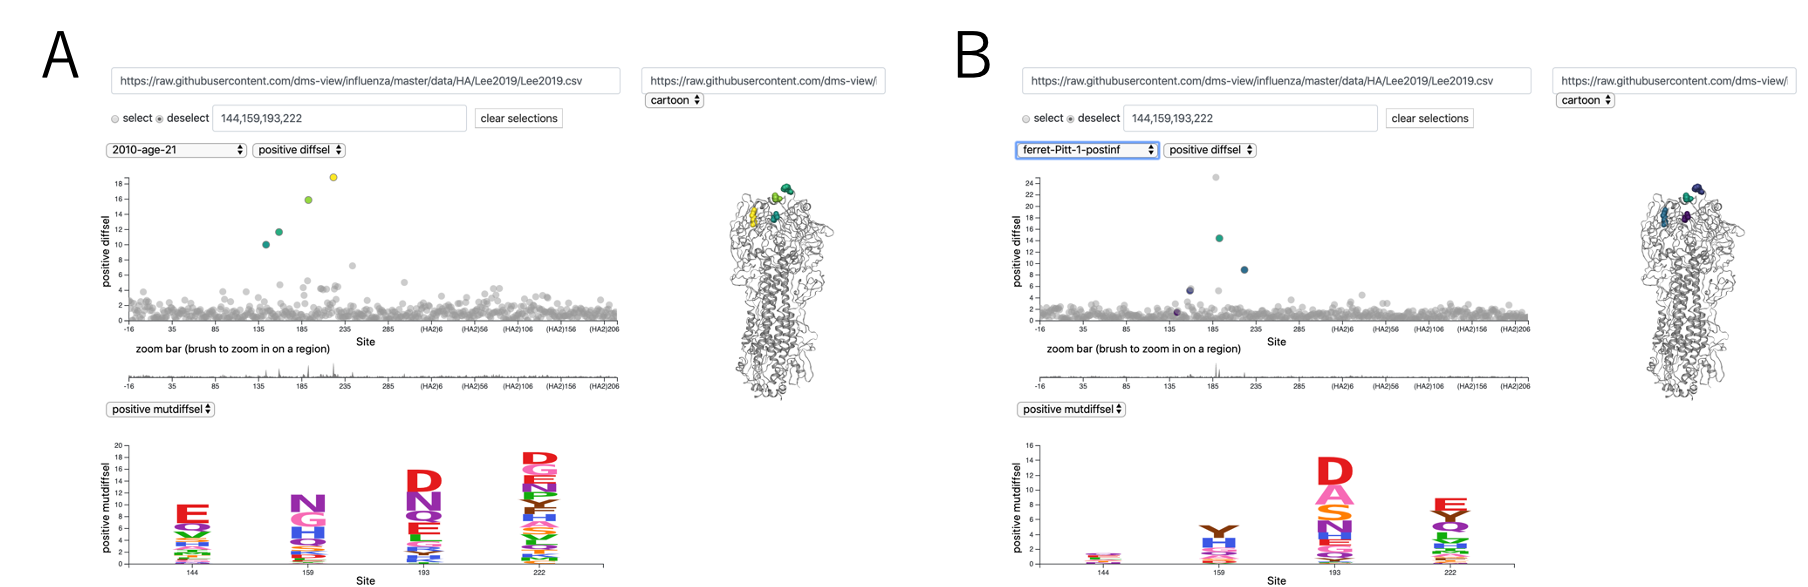
\includegraphics[width=0.90\textwidth]{../fig/human-vs-ferret.png}}
\caption[Comparing sites targeted by human sera to sites targeted by ferret sera.]{
\label{fig:human-vs-ferret}
{\bf (A)} We selected the sites most highly targeted by the human sera ``2010-age-21", sites 144, 159, 193, and 222. The selected sites are colored in the site dot plot, highlighted on the protein structure, and the full mutation-level information is shown in the logoplot.
{\bf (B)} We changed the \textit{condition} dataset from the human sera ``2010-age-21" to the ferret sera ``ferret-Pitt-1-postinf".
The sites selected in (A) remain selected in (B).
}
\end{figure}
